%Figure list:
% Vsup vs. traditional 2D heatmap vs. juxtaposed maps
% Chart of color bins w/r/t CIELAB threshold, with iconic maps at intervals
% Process figure
% Real examples with different color maps

\newcommand{\exampleFig}{
\begin{figure}[t]
	\centering
	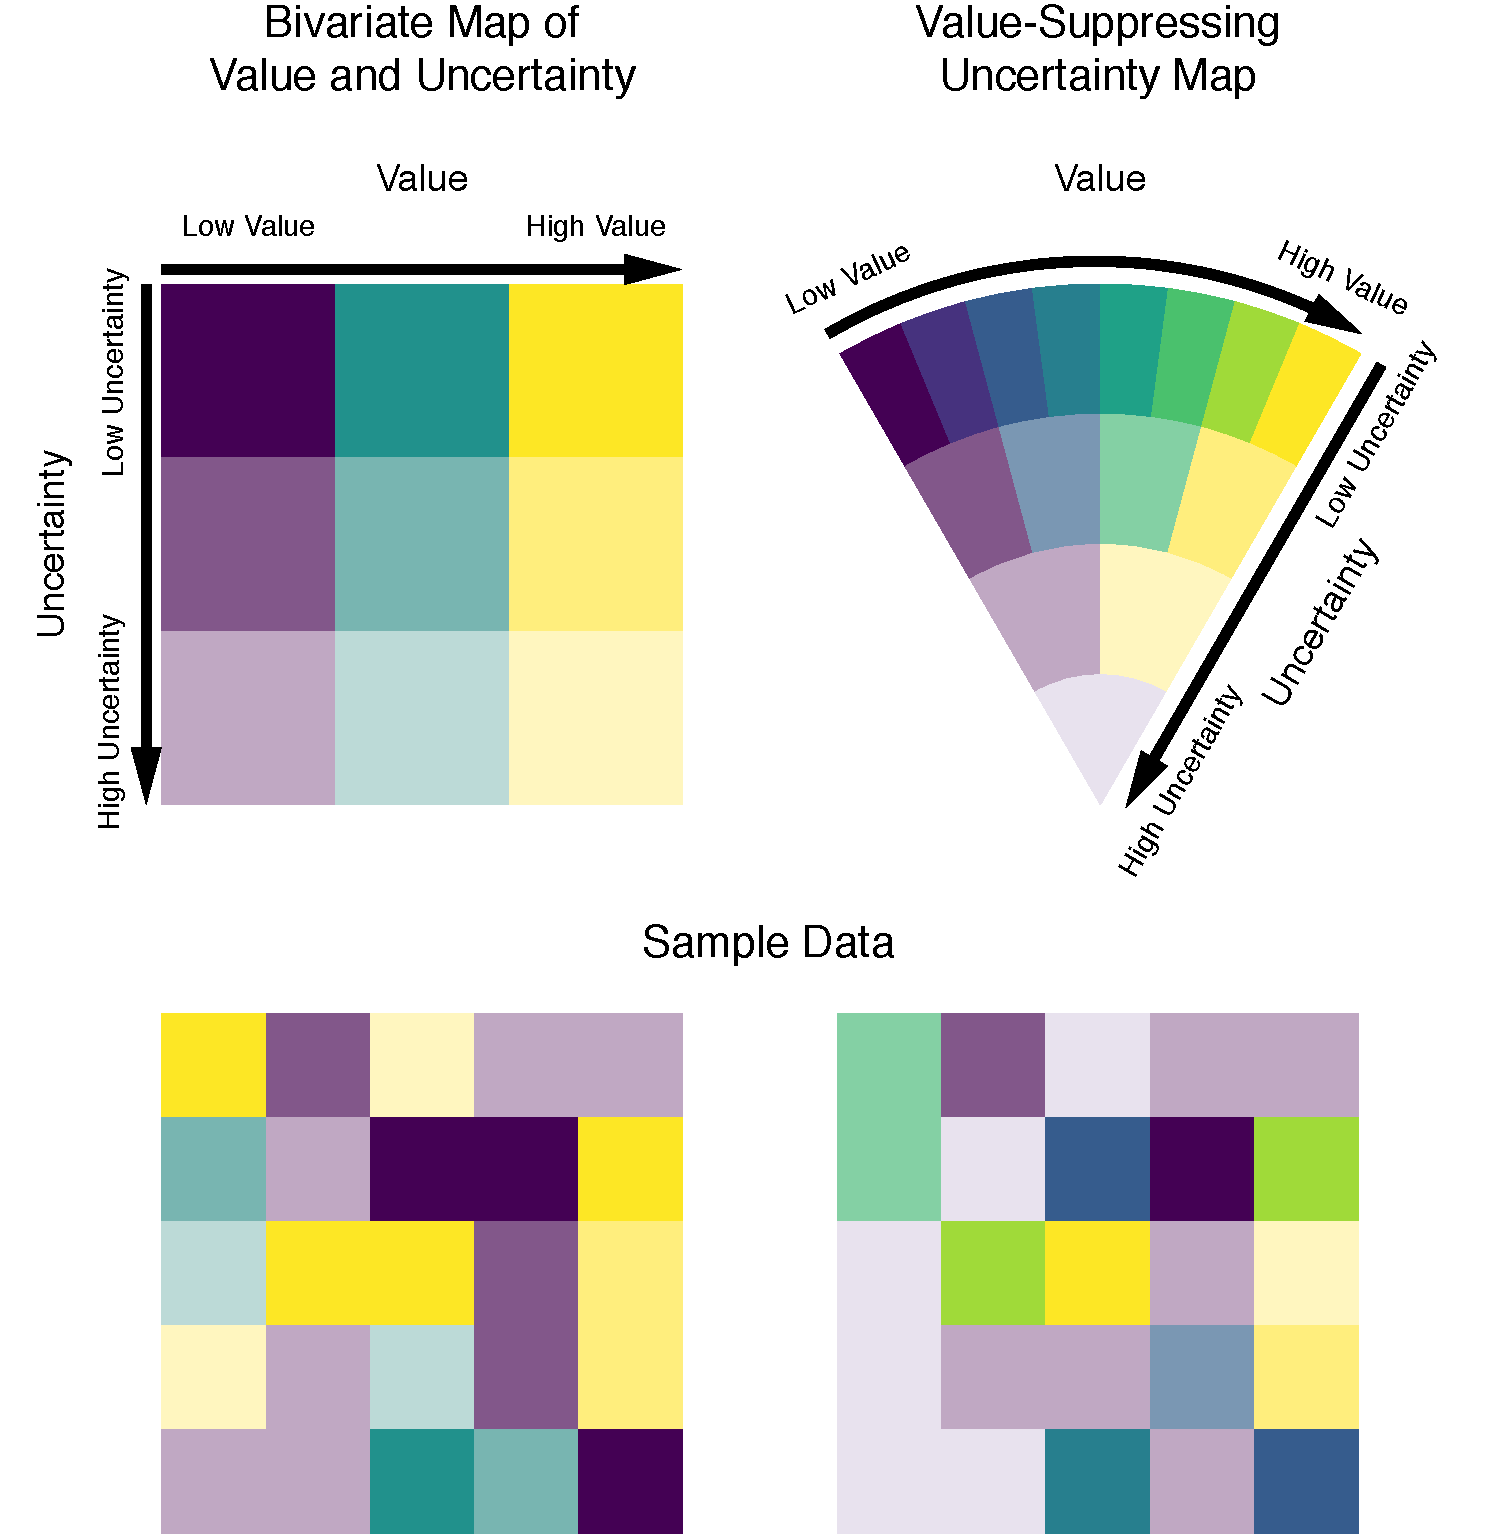
\includegraphics[width=0.9\columnwidth]{example.pdf}
	\caption{A standard bivariate map (left) and a VSUP (right), used to encode an identical 10x10 grid of random data. Both use the same visual channels to encode value (position along the Viridis~\protect\cite{viridis} color map) and uncertainty (lightness and saturation). However, the VSUP uses a tree-like structure to allocate colors, defining more bins when uncertainty is low. This non-uniform budgeting affords better discrimination between values when uncertainty is low, even though the VSUP has fewer color bins (in this case, 15 to the bivariate map's 16). This tree-like structure also discourages analysis in regions where uncertainty may be unacceptably high.}
	\label{fig:example}
\end{figure}
}

\newcommand{\sizeFig}{
	\begin{figure}
		\centering
		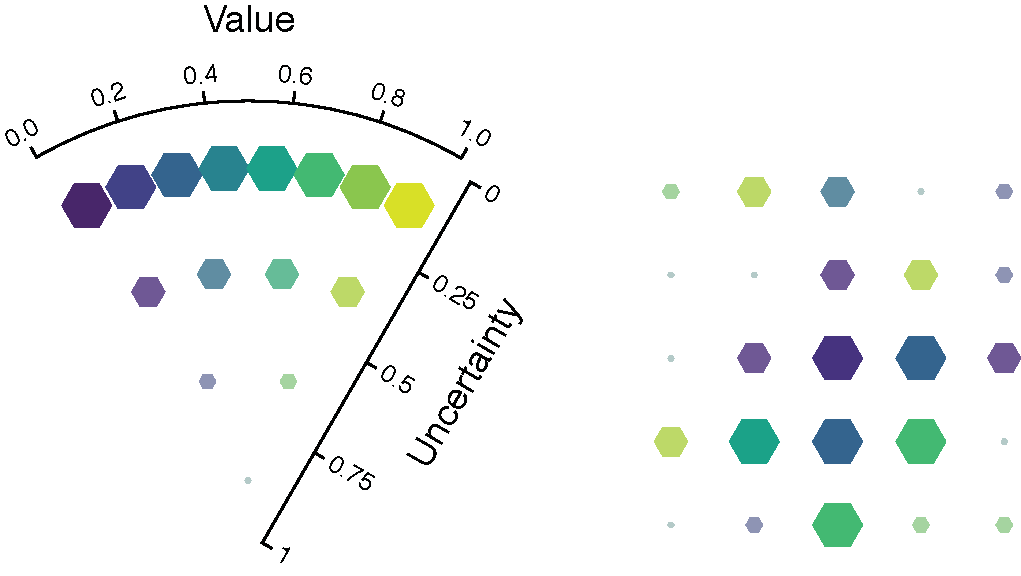
\includegraphics[width=0.9\columnwidth]{size.pdf}
		\caption{A VSUP where value is mapped to color, and uncertainty is mapped to glyph area. As glyphs become smaller, it becomes more difficult to distinguish their colors~\protect\cite{stone2014engineering}. VSUPs, by reducing the number of color categories as uncertainty increases, account for this ambiguity. On the right, the VSUP has been used to encode a 5x5 grid of random data.}
		\label{fig:size}
	\end{figure}
}

\newcommand{\conditionFig}{
	\begin{figure*}[t]
		\centering
		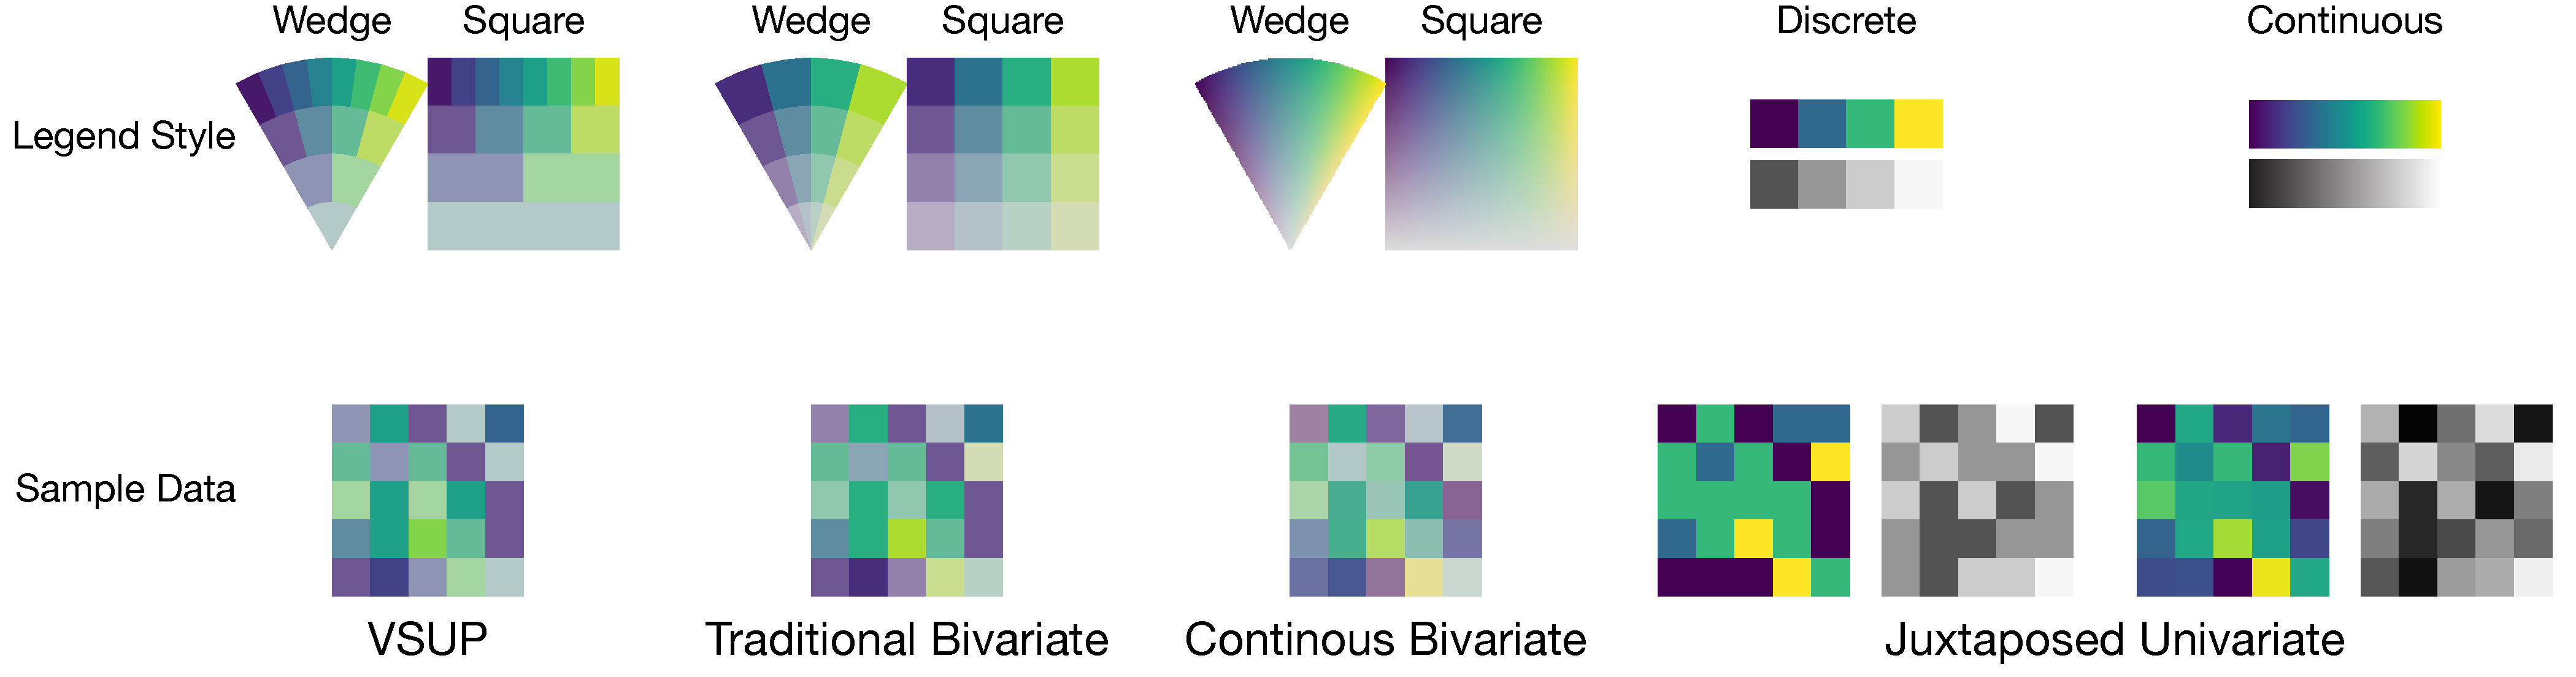
\includegraphics[width=0.95\textwidth]{allConditions.pdf}
		\caption{The 8 conditions from the identification experiment. Juxtaposed maps require a participants to make an error-prone connection between areas in two separate maps in order to make a decision that integrates value and uncertainty. Traditional bivariate maps integrate both value and uncertainty. VSUPs attempt to improve on traditional bivariate maps by reducing color resolution as uncertainty increases, discouraging conclusions based on noisy or imprecise data.}
		\label{fig:conditions}
	\end{figure*}
}

\newcommand{\taskOneFig}{
	\begin{figure}
		\centering
		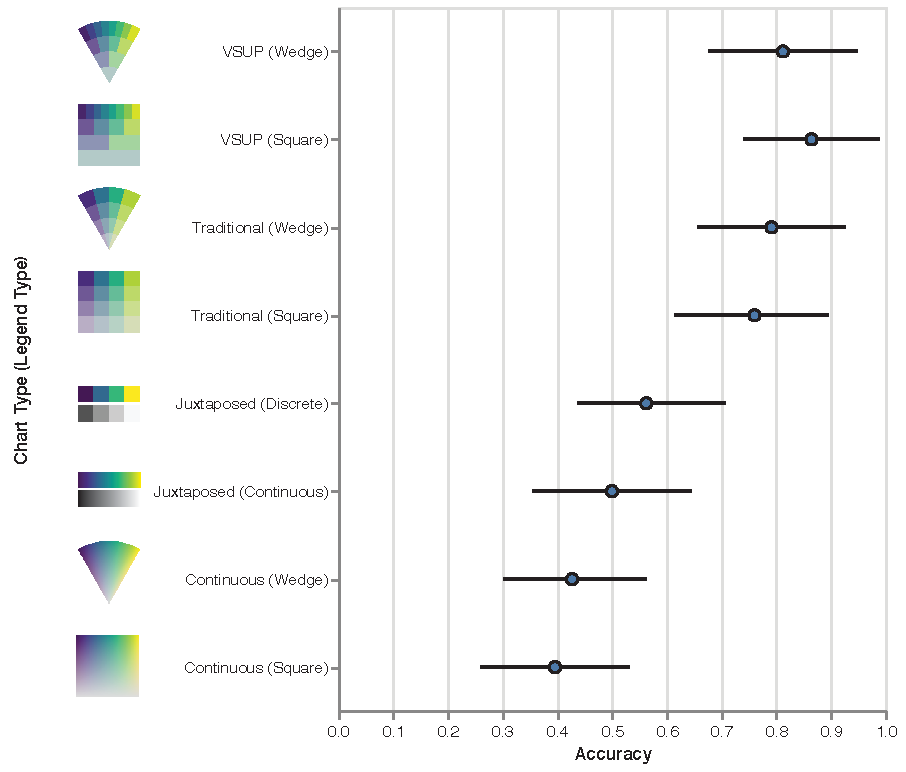
\includegraphics[width=0.95\columnwidth]{task1.pdf}
		\caption{Accuracy results for the identification experiment. For examples of each condition, see \protect\figref{fig:conditions}. Juxtaposing two univariate maps for both value and uncertainty requires an error-prone search task for identification tasks. Continuous rather than discrete bivariate maps requires an error-prone color encoding and estimation task. Discrete bivariate maps, both VSUPs and otherwise, avoid these issues. The confidence intervals are bootstrapped 95\% CIs of trimmed means.}
		\label{fig:taskOne}
	\end{figure}
}

\newcommand{\taskTwoFig}{
	\begin{figure}
		\centering
		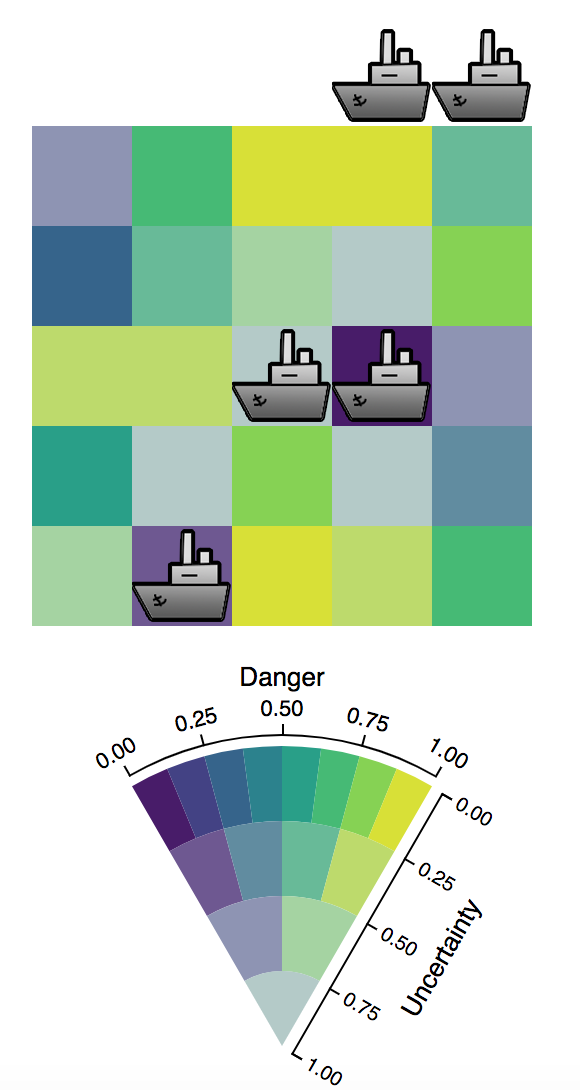
\includegraphics[width=0.4\columnwidth]{defend.png}
		\caption{The prediction task. The participant has a list of locations, and ought to place their ships on locations with low probability of attack, and high certainty in this probability. Ships above the heatmap have yet to be placed.}
		\label{fig:taskTwoConditions}
	\end{figure}
}

\newcommand{\taskTwoViolin}{
	\begin{figure}
		\centering
		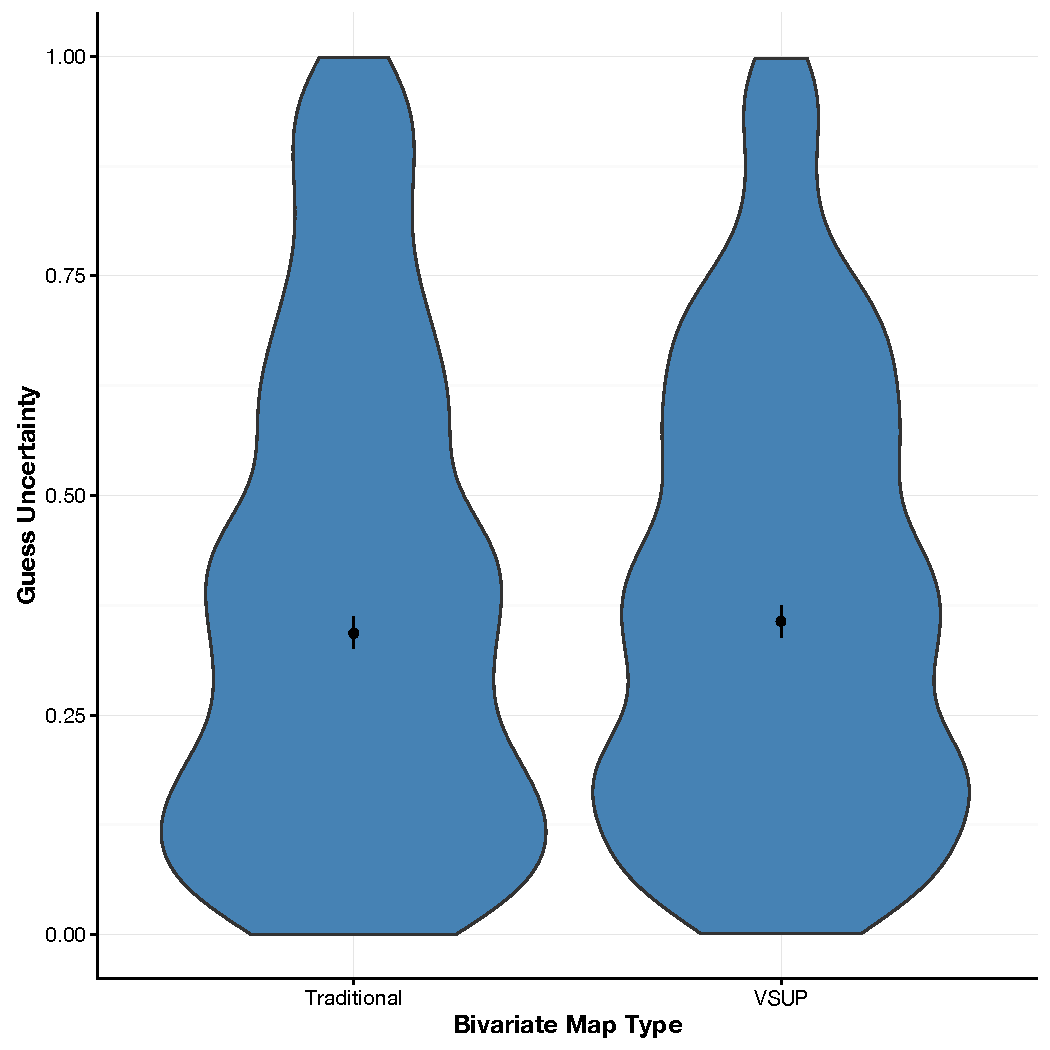
\includegraphics[width=0.75\columnwidth]{violin.pdf}
		\caption{A violin plot of results from our prediction experiment. While, on average, participants selected squares with similar uncertainty overall, participants using VSUPs were dissuaded from making guesses with high uncertainty, instead spreading their risk over other categories. The confidence intervals are bootstrapped 95\% CIs of trimmed means.}
		\label{fig:taskTwoViolin}
	\end{figure}
}

\newcommand{\taskTwoHeatmap}{
	\begin{figure}
		\centering
		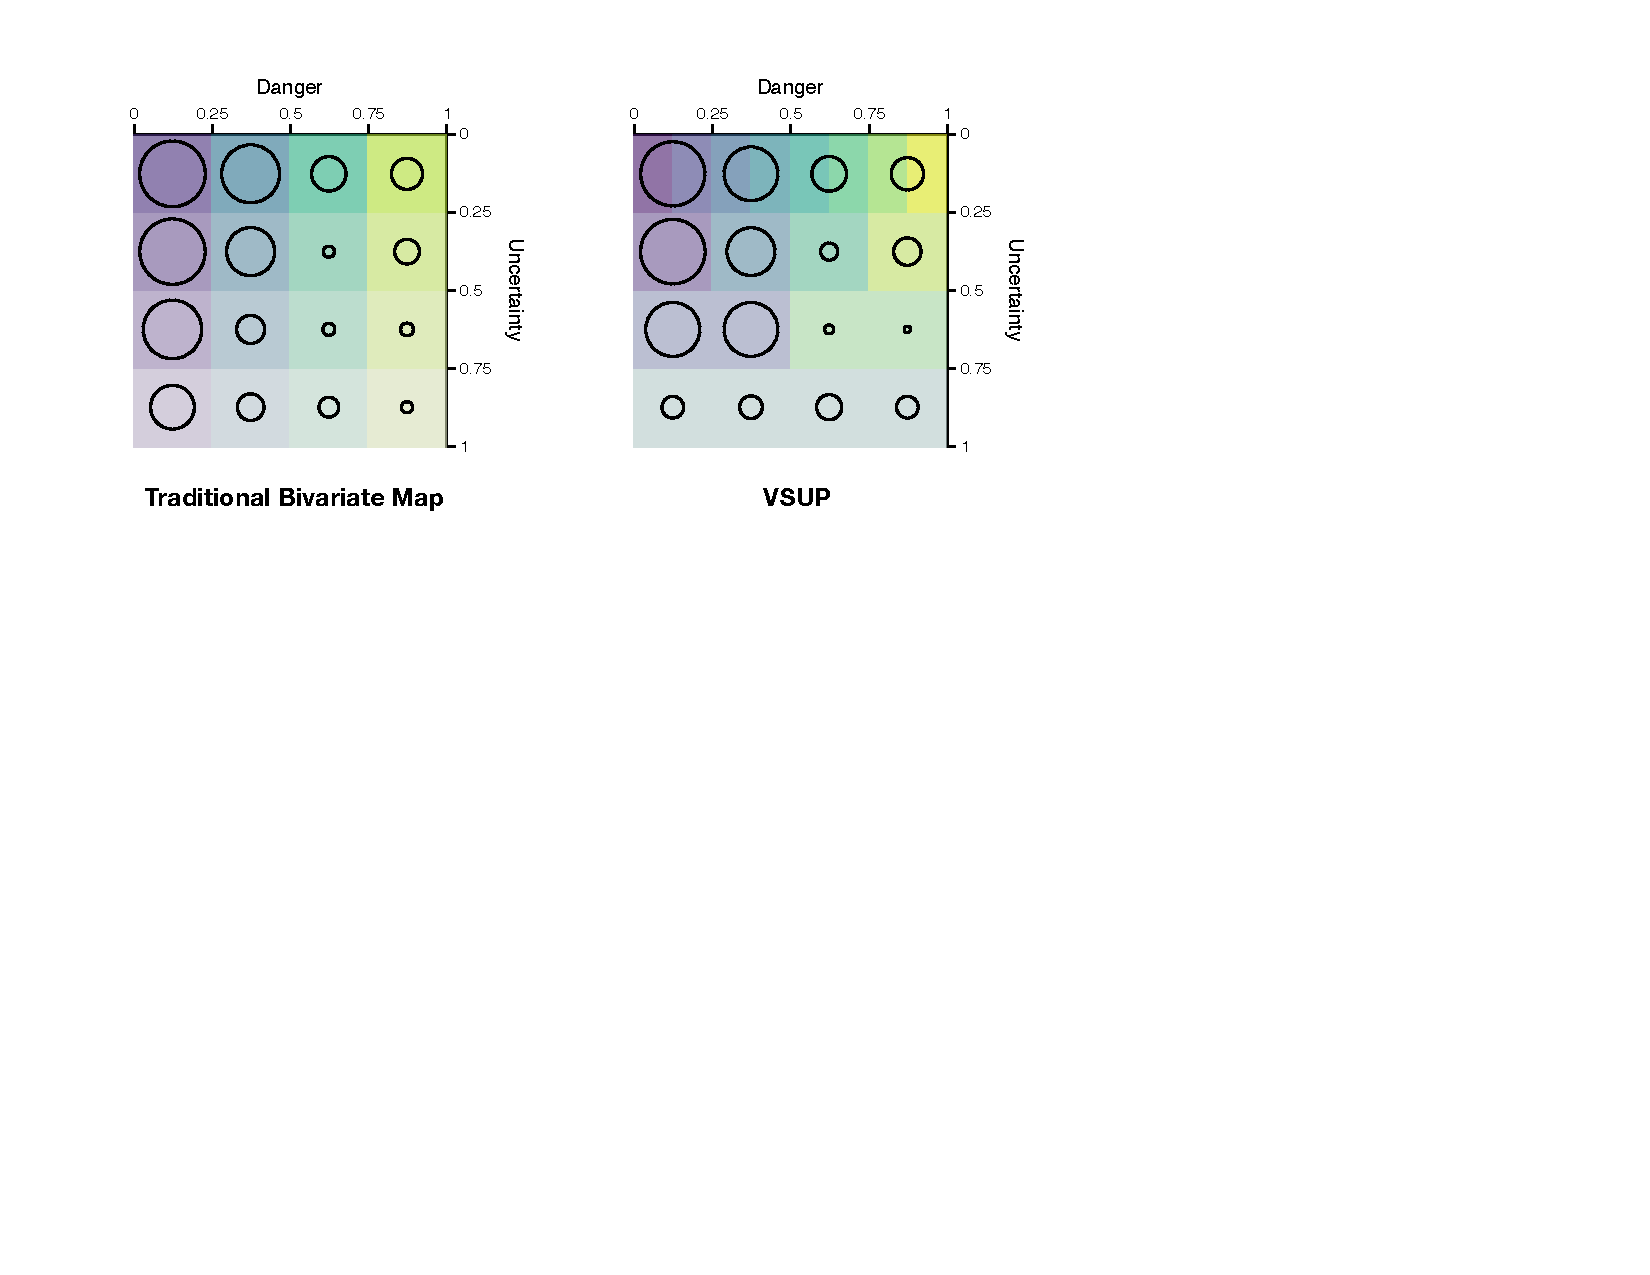
\includegraphics[width=0.9\columnwidth]{exp2histogram.pdf}
		\caption{2D histogram of placements from the prediction experiment. For each trial, participants were asked to place 5 tokens on heatmaps encoding both predicted safety, and uncertainty in these predictions. There were intentionally more tokens to place than there were ``safe and certain'' locations (top left corner). When looking at traditional 2D maps (left), participants favored safe but uncertain locations (bottom left corner). When looking at VSUPs (right), participants favored locations that were less safe, but more certain.)}
		\label{fig:taskTwoHeatmap}
	\end{figure}
}
%\newcommand{\performanceFig}{
%	\begin{figure}[t]
%		\centering
%		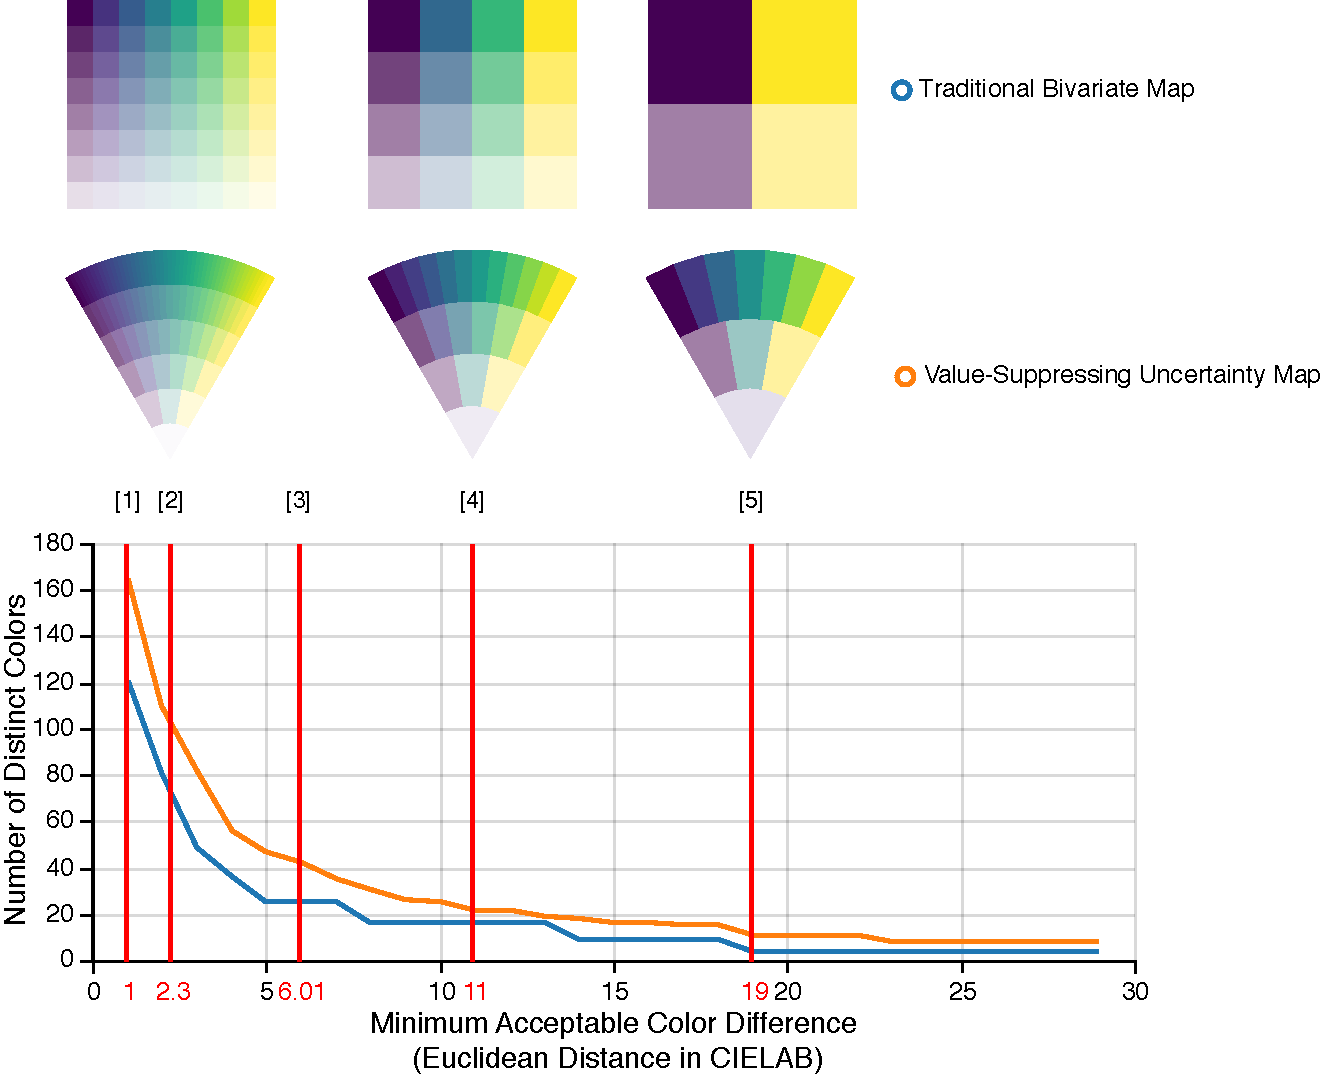
\includegraphics[width=0.9\columnwidth]{performance.pdf}
%		\caption{
%			The number of discrete color categories in traditional bivariate color maps versus VSUPs, assuming value is encoded by the Viridis color map~\protect\cite{viridis}, and uncertainty is encoded by saturation/value (whiter values are more uncertain). Since these whiter uncertain colors are closer together in CIELAB space, and VSUPs intentionally require fewer color bins in those regions, VSUPs always have more color categories than the corresponding 2D bivariate map. The red lines denote:
%		  \textbf{1)} Theoretical 50\% JND from CIELAB specification.
%			\textbf{2)} 50\% JND from controlled lab study of Mahy et al.~\protect\cite{mahy1994evaluation}.
%			\textbf{3)} 50\% JND from Szafir et al.\protect\cite{szafir2014adapting}.
%			\textbf{4)} 50\% JND for small visual targets from Stone et al.~\protect\cite{stone2014engineering}.
%			\textbf{5)} The threshold resulting in the simplest possible (2x2) bivariate map.
%	    }
%		\label{fig:performance}
%	\end{figure}
%}

%\newcommand{\flowFig}{
%	\begin{figure}[t]
%		\centering
%		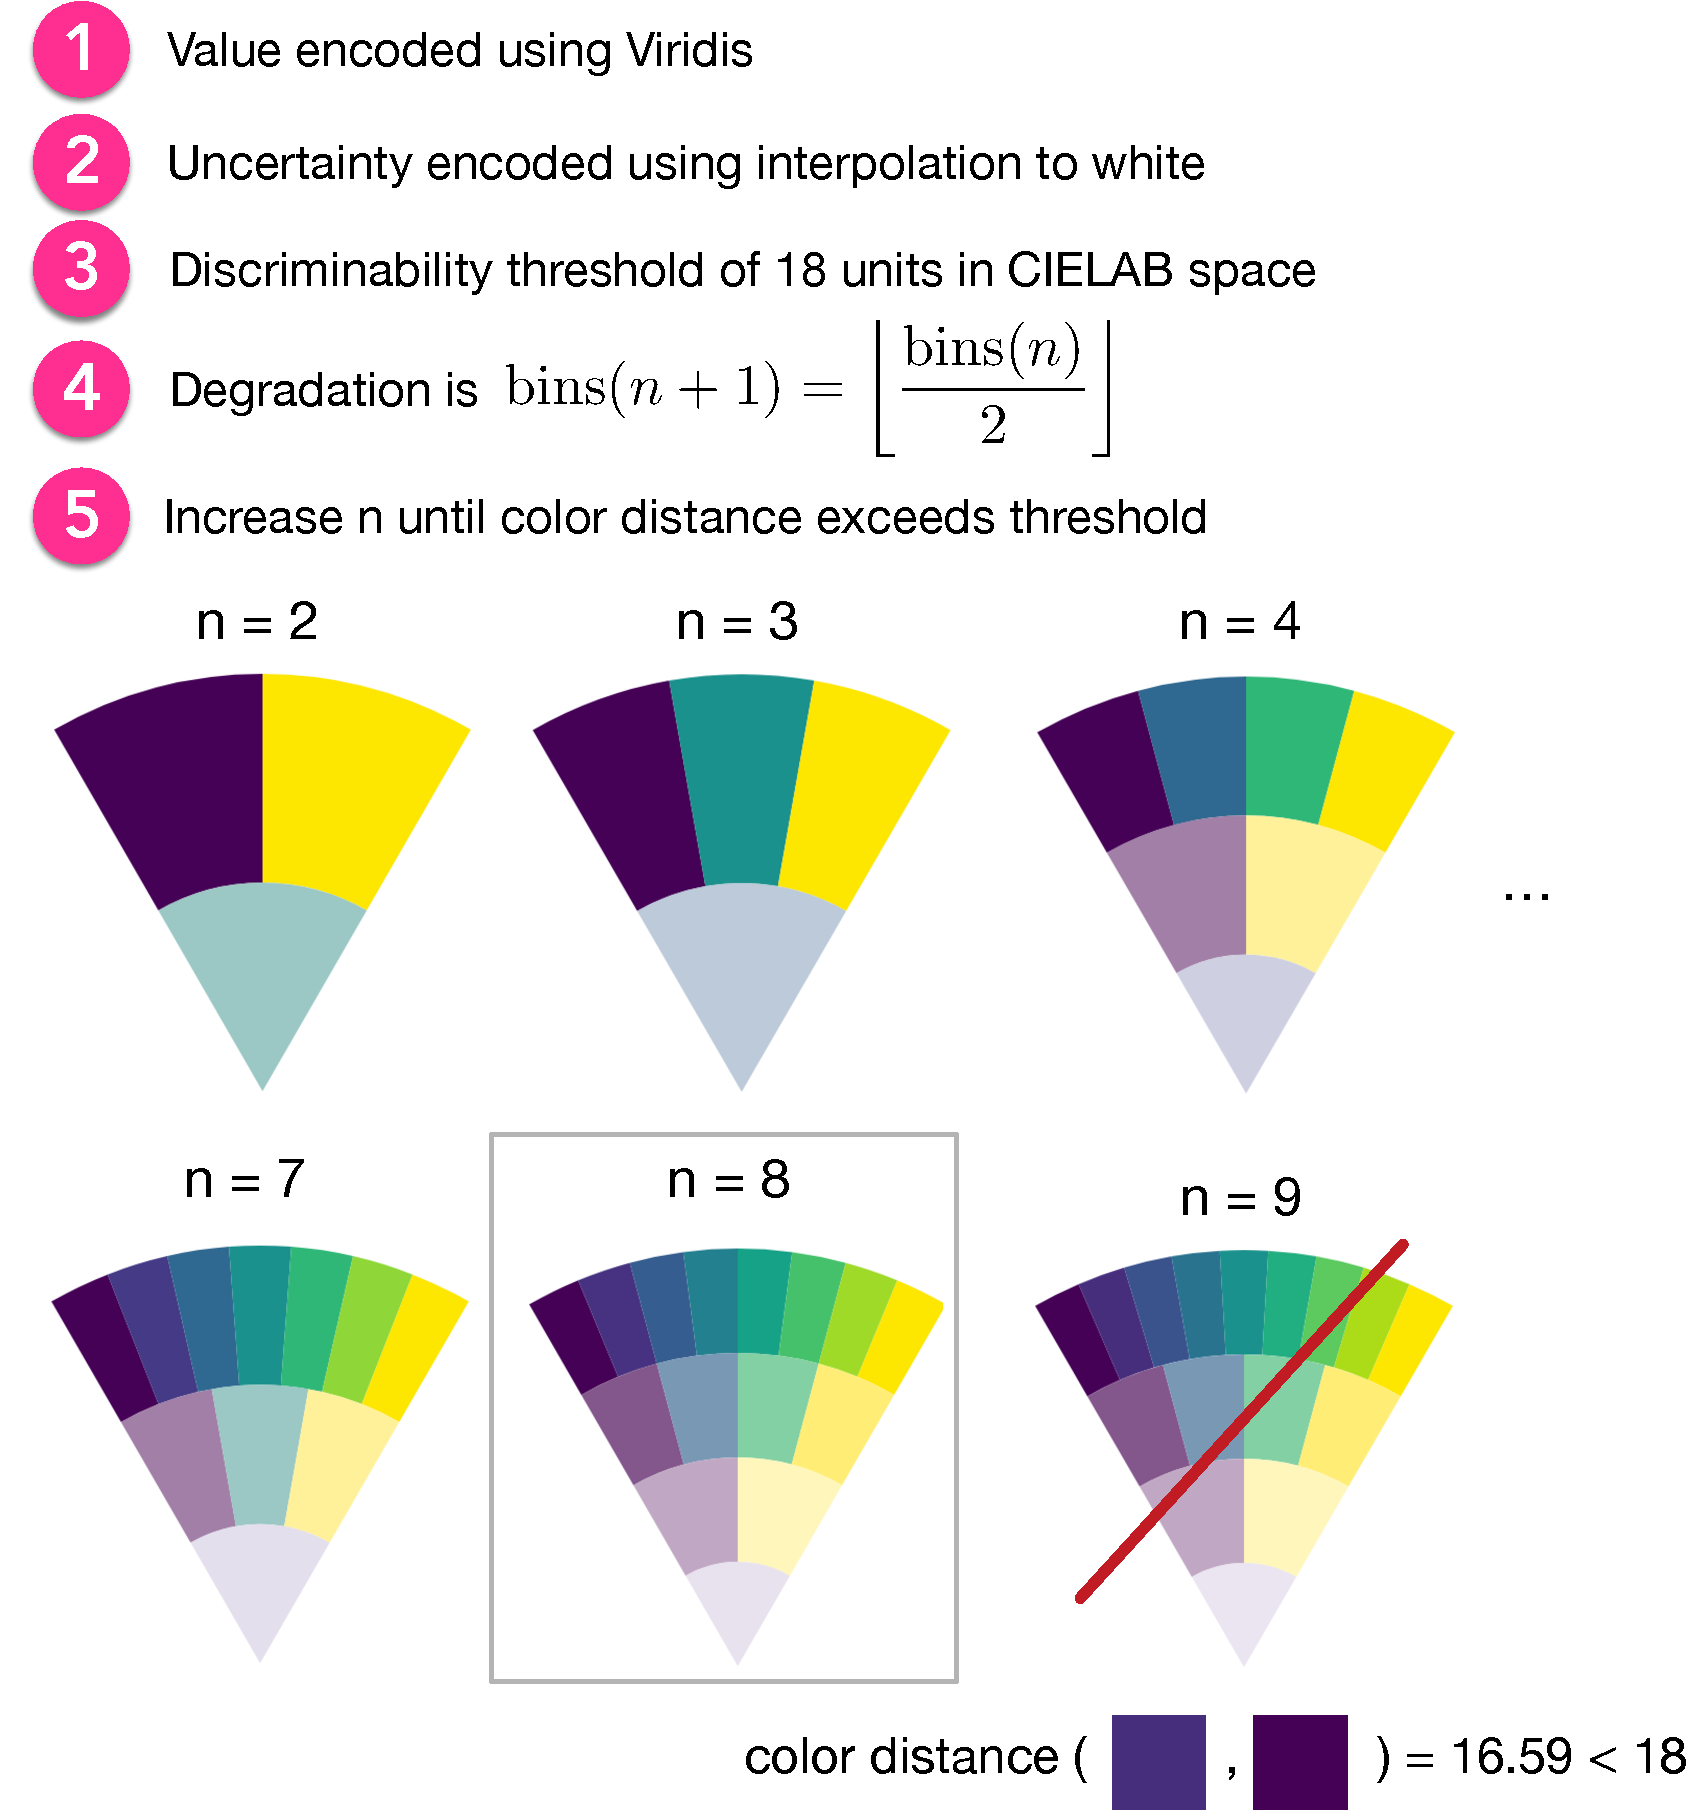
\includegraphics[width=0.95\columnwidth]{flow.pdf}
%		\caption{The process for creating a VSUP. VSUPs guarantee that no two marks in the resulting bivariate mapping are perceptually closer than some pre-specified threshold. This guarantee removes some of the issues of non-separability and ambiguity that are otherwise a concern when designing bivariate maps. \\
%		In this example two colors from the map for $n=9$ are too close in CIELAB space. Thus, we create a VSUP with $n=8$ color bins at the lowest level of uncertainty.}
%		\label{fig:flow}
%	\end{figure}
%}

\newcommand{\airlineFig}{
\begin{figure}[t]
	\centering
	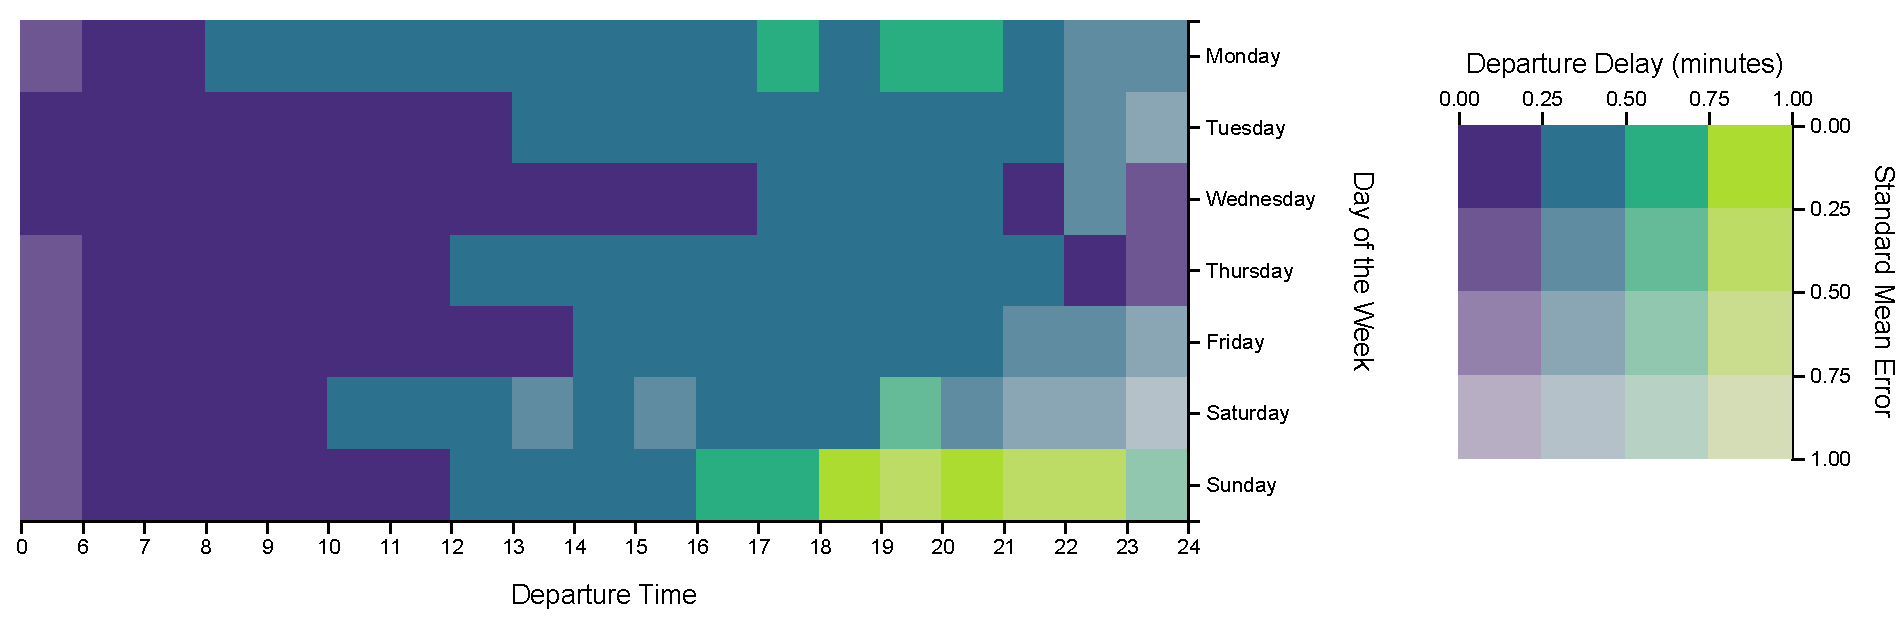
\includegraphics[width=\columnwidth]{airline-2d}
	\vspace{-15px}
	\caption{Average departure delay for different times of the day and days of the week visualized with a 2D uncertainty map. Horizontal position is the hour of scheduled departure, and vertical position is the day of the week.}
	\label{fig:airline2d}

	\vspace{10px}

	\centering
	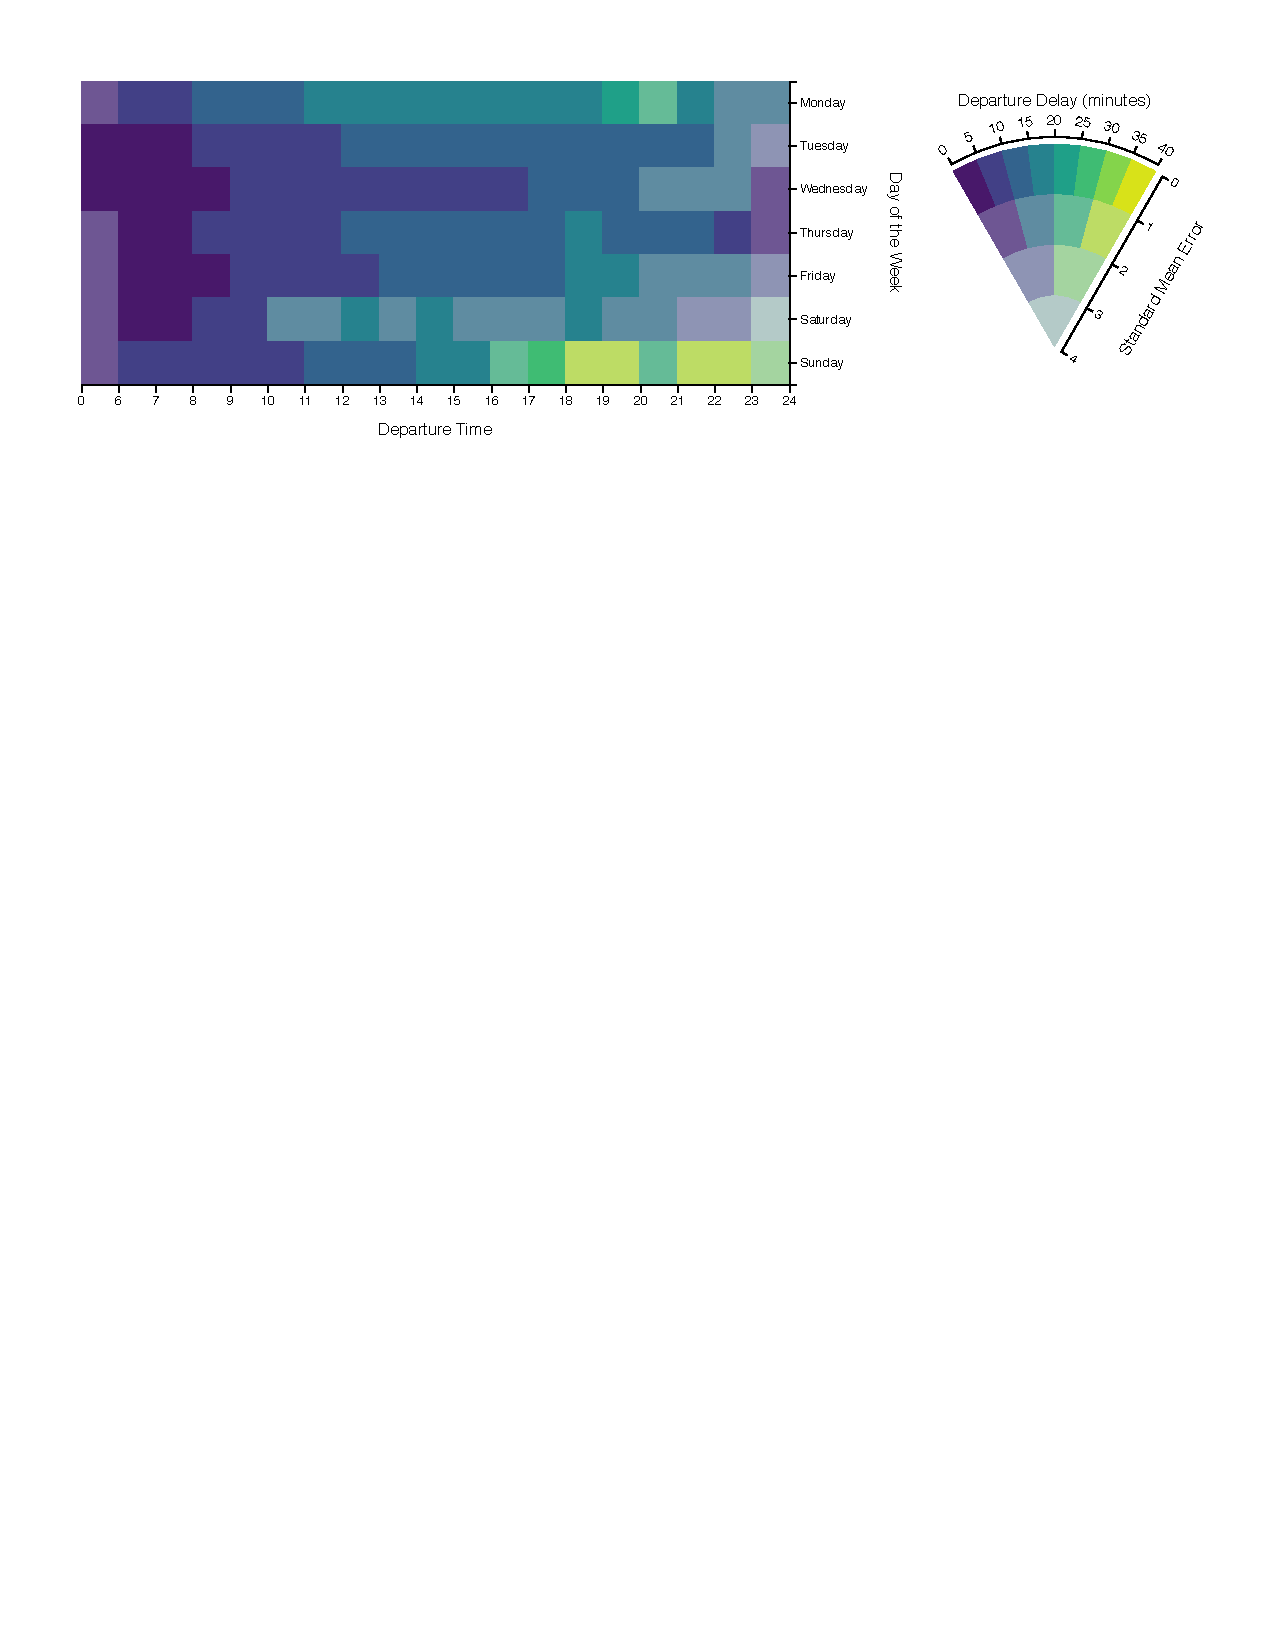
\includegraphics[width=\columnwidth]{airline-vsup}
	\vspace{-15px}
	\caption{Flight delay data encoded with a VSUP.}
	\label{fig:airlineVsup}
\end{figure}
}

\newcommand{\viralFig}{
\begin{figure}[t]
	\centering
	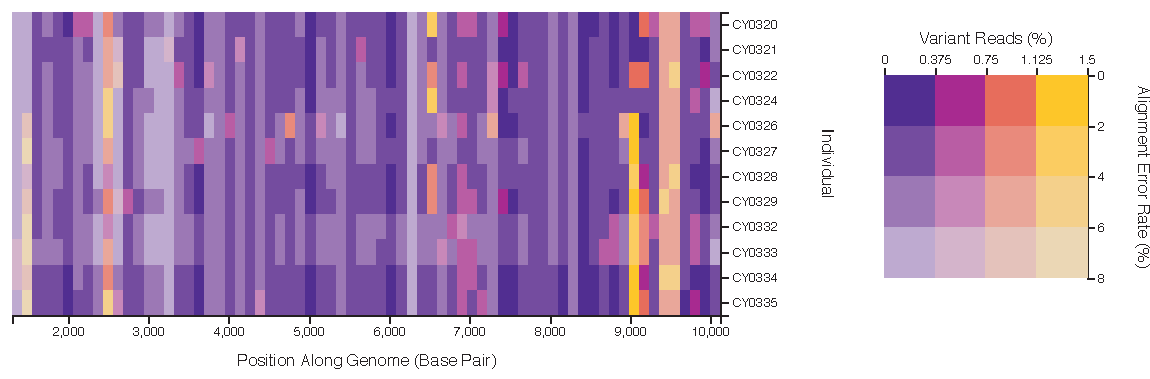
\includegraphics[width=\columnwidth]{viral-2d.pdf}
	\vspace{-15px}
	\caption{Variability for 12 different viral populations of the SIV virus, encoded with a traditional 2D bivariate map. Horizontal position denotes location along the SIV genome. Each row is the viral population of a different infected animal. Error in aligning short reads can lead to poor quality data, and so the amount of these errors is encoded as the uncertainty. }
	\label{fig:viral2d}

	\vspace{10px}

	\centering
	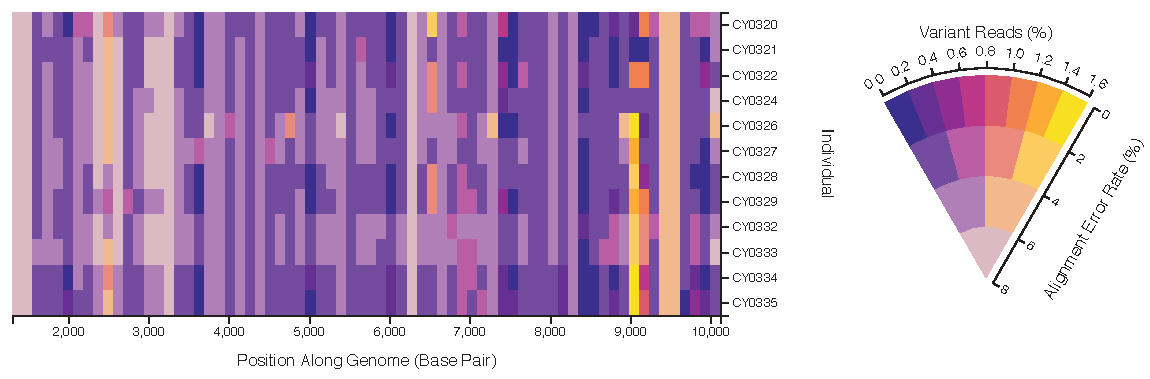
\includegraphics[width=\columnwidth]{viral-vsup.pdf}
	\vspace{-15px}
	\caption{Variability for 12 different viral populations of SIV, encoded with a VSUP. By suppressing uncertain information, the VSUP version removes the apparent spike in value at the second column, which is an artifact of sampling error due to poor coverage in that region. It also suppresses apparent inter-species variability in the solid orange spike at location ~9,500, which, again, is a function of poor coverage rather than a genuine per-strain difference.  }
	\label{fig:viralVsup}
\end{figure}
}

\newcommand{\pollFig}{
	\begin{figure}[t]
		\centering
		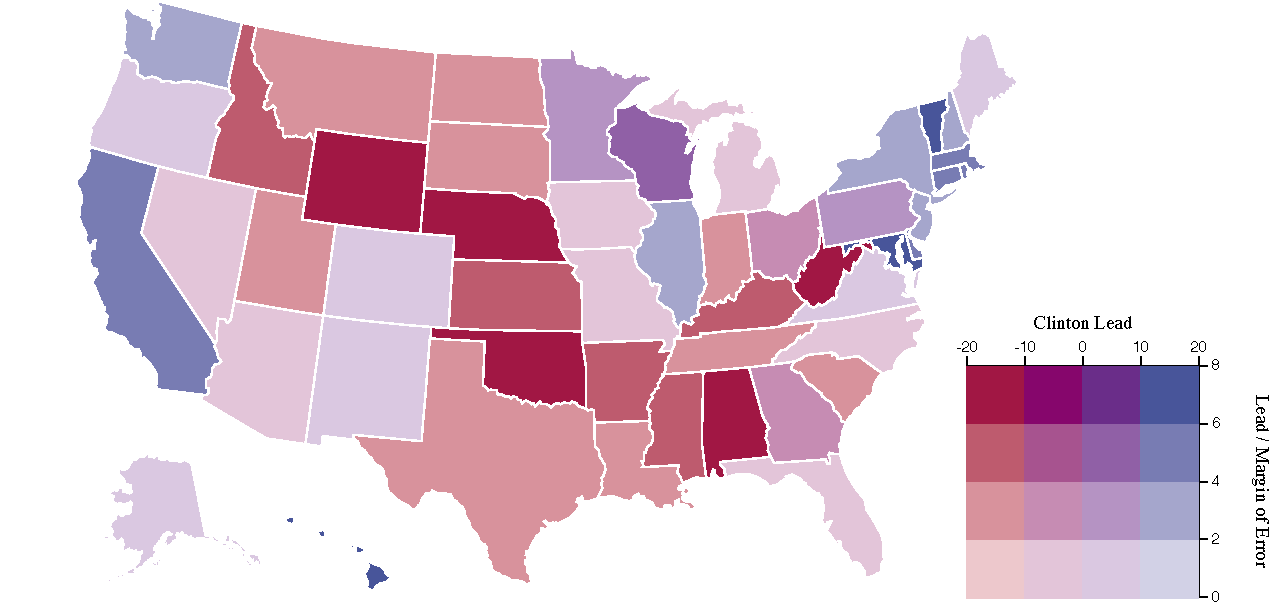
\includegraphics[width=\columnwidth]{polling-2d.pdf}
		\vspace{-15px}
		\caption{Polling data prior to the 2016 U.S. Presidential Election, encoded in a traditional 2D bivariate map. The redness and blueness show the polling lead for Trump and Clinton, respectively. But many polls had high margins of error, creating uncertainty about the election results.}
		\label{fig:polling2d}
		
		\vspace{10px}
		
		\centering
		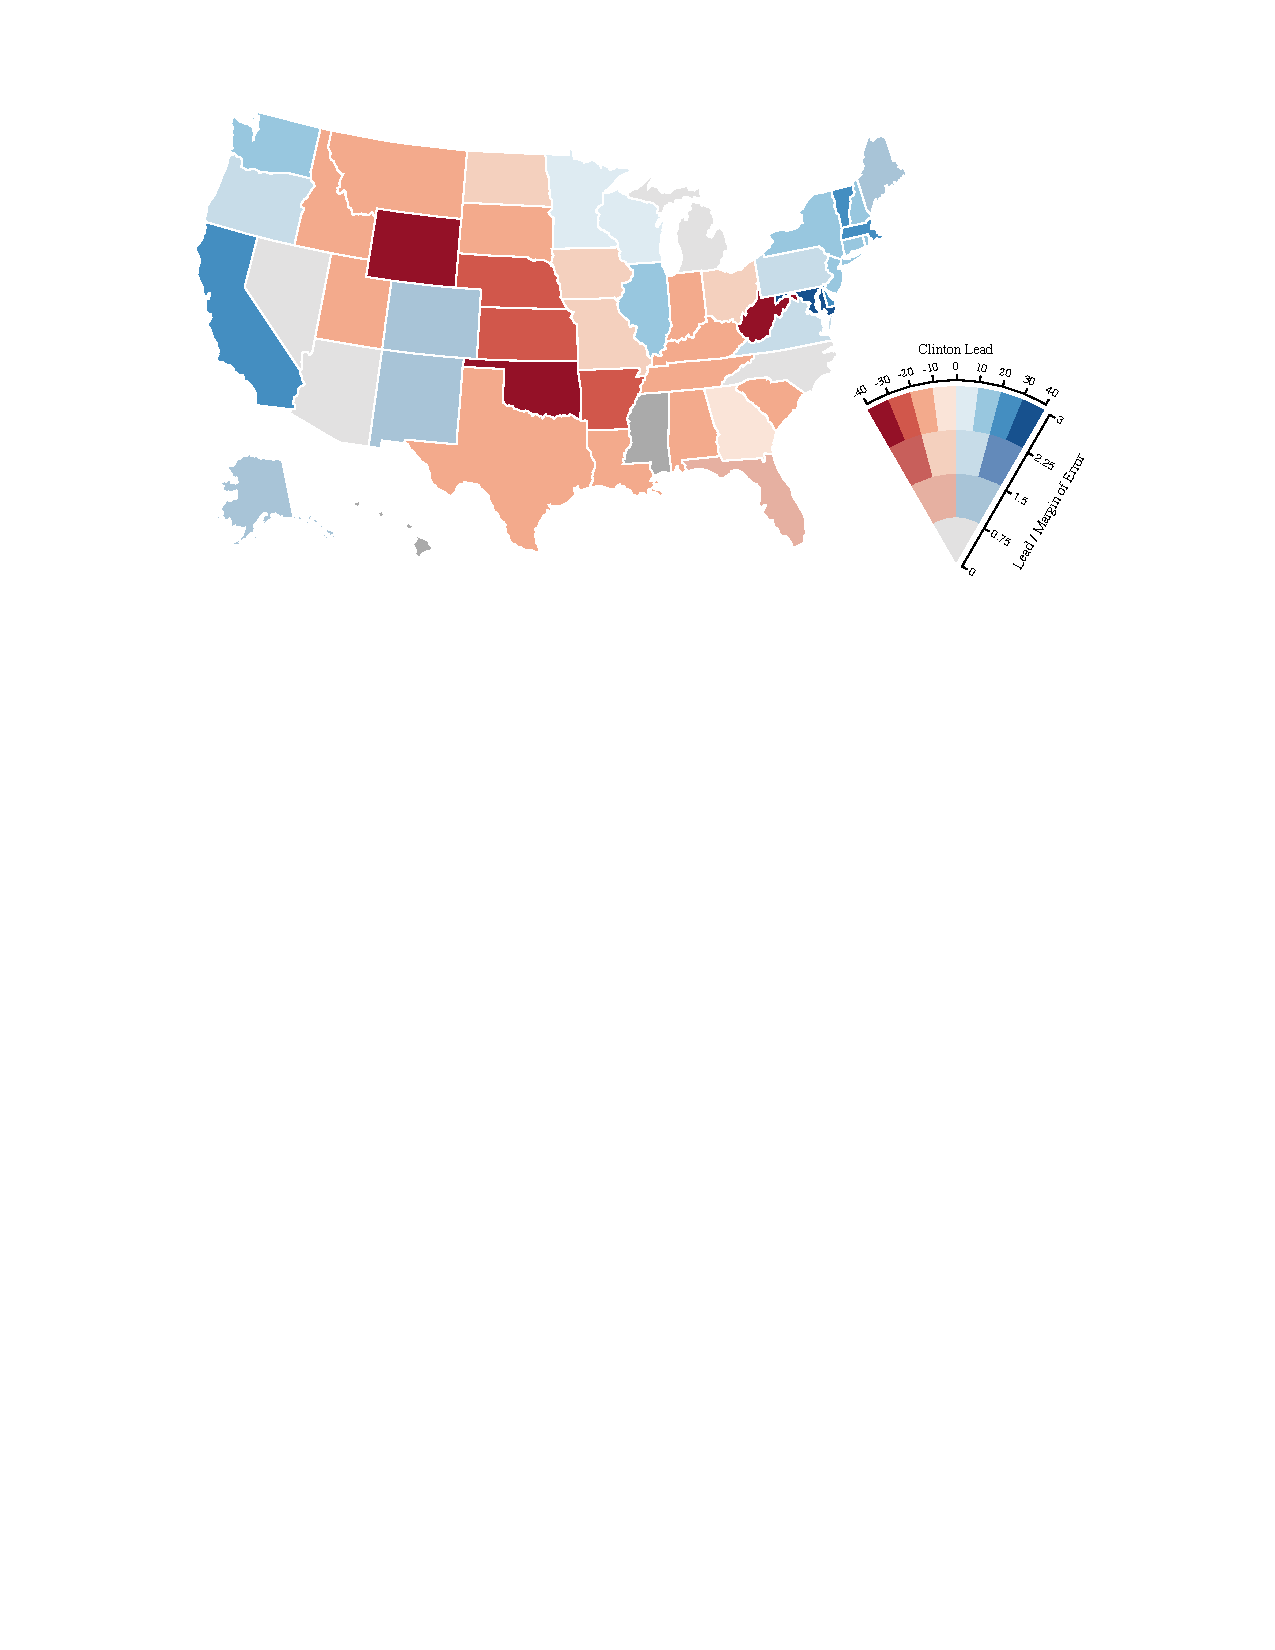
\includegraphics[width=\columnwidth]{polling-vsup.pdf}
		\vspace{-15px}
		\caption{Polling data prior to the 2016 U.S. Presidential Election, encoded with a VSUP. }
		\label{fig:pollingVsup}
	\end{figure}
}

\newcommand{\responseTimeFig}{
	\begin{figure}[t]
		\centering
		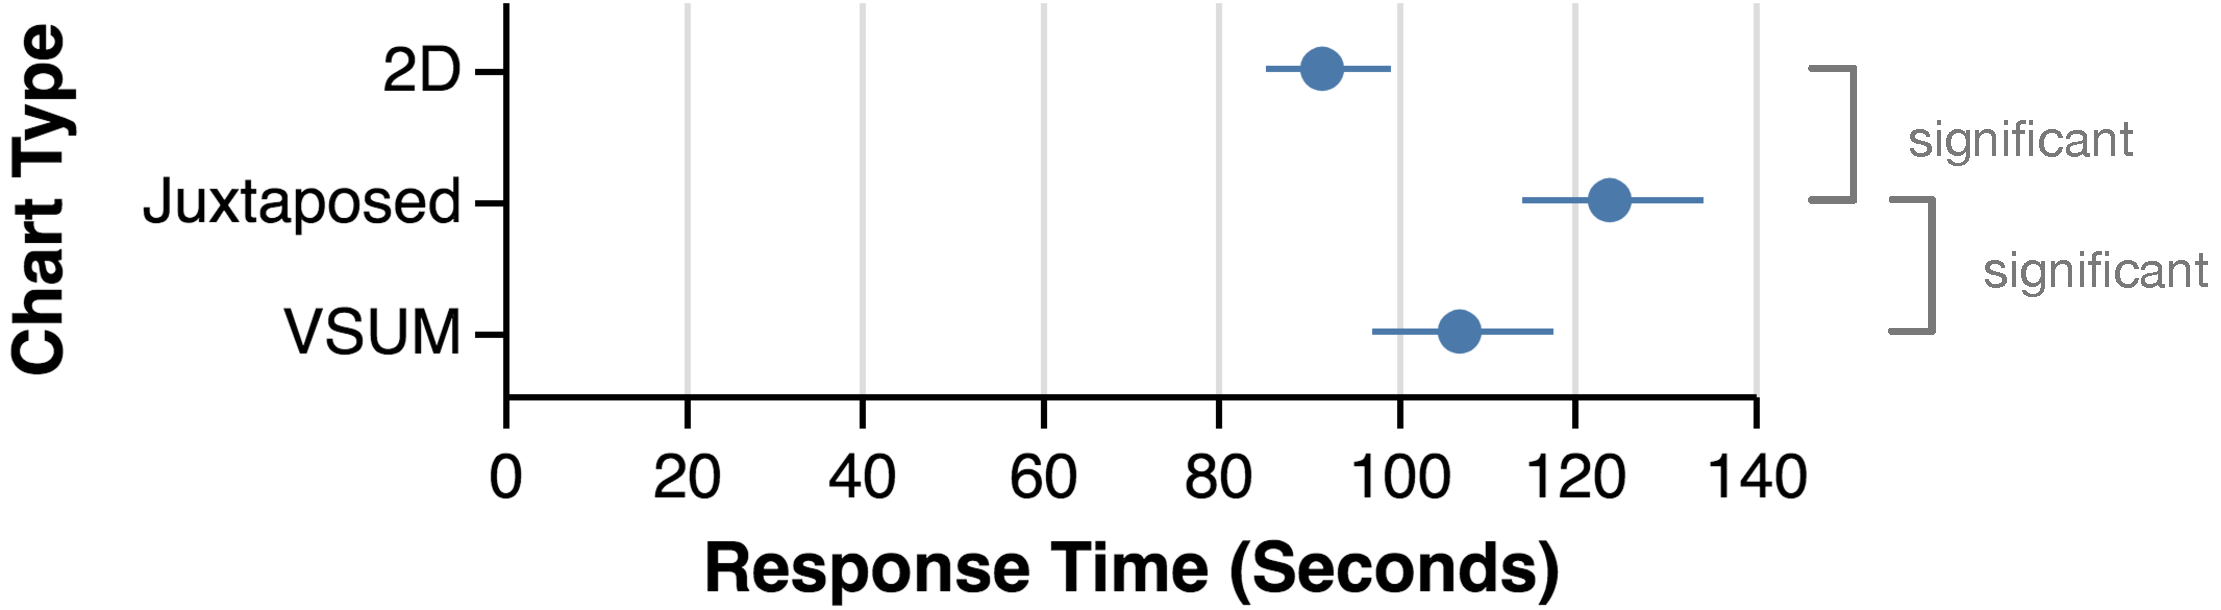
\includegraphics[height=2.4cm]{rt1.pdf}
		\caption{The effect of chart type on response time for the identification task. Juxtaposed maps of value and uncertainty introduce a visual search task, increasing the time to complete even simple tasks involving both value and uncertainty information. The confidence intervals are bootstrapped 95\% CIs of trimmed means.}
		\label{fig:rt1}
	\end{figure}
}

\newcommand{\accuracyFig}{
	\begin{figure}[t]
		\centering
		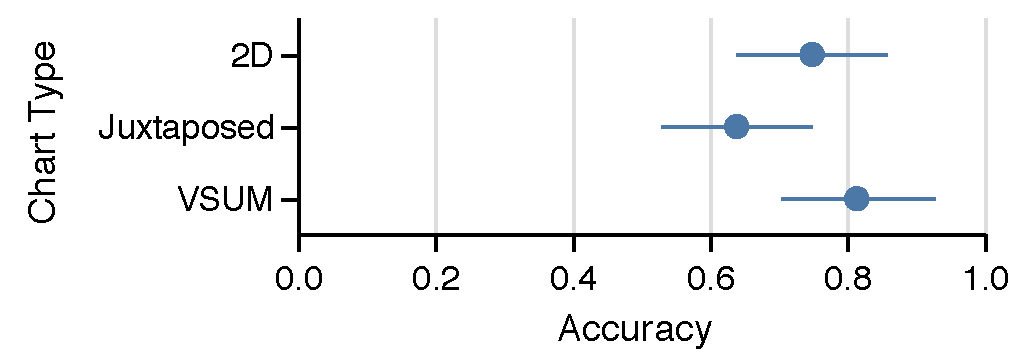
\includegraphics[height=2.4cm]{accuracy1.pdf}
		\caption{The effect of chart type on accuracy for the identification task. VSUPS are similarly accurate for simple search tasks as more traditional bivariate visualizations, despite containing additional colors categories, and having a more complex relationship between uncertainty, value, and color than traditional charts. The confidence intervals are bootstrapped 95\% CIs of trimmed means.}
		\label{fig:accuracy1}
	\end{figure}
}

\newcommand{\uncertaintyFig}{
	\begin{figure}[t]
		\centering
		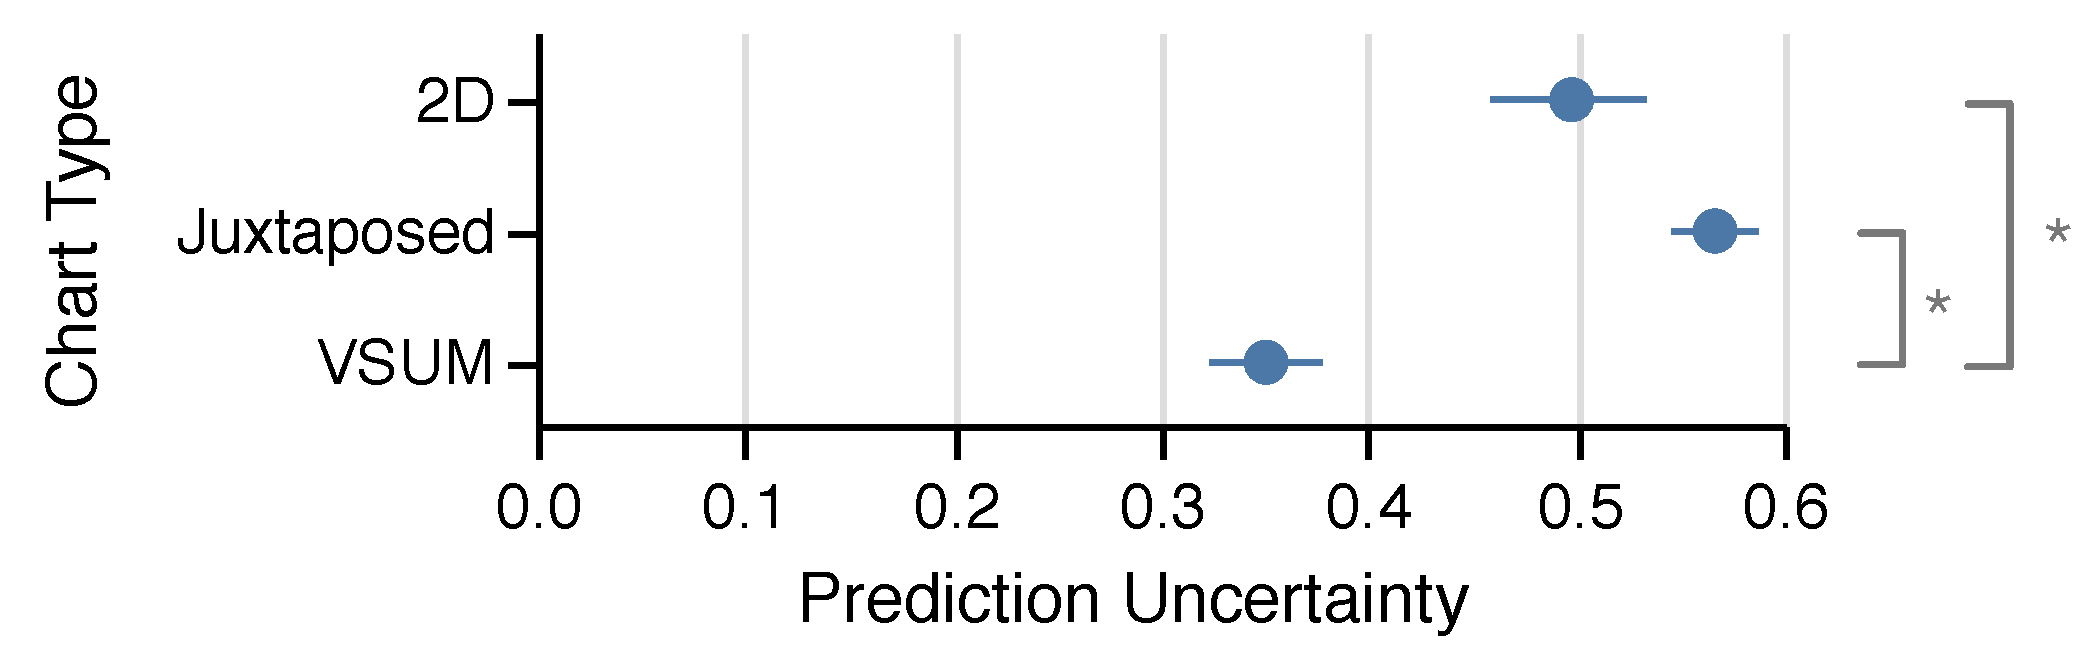
\includegraphics[height=2.4cm]{uncertainty2.pdf}
		\caption{The effect of chart type on the average uncertainty in predictions for the prediction task. By reducing the number of color categories as uncertainty increases, VSUPs encourage more caution in predictions, making people less likely to consider data with strong, but spurious patterns. The confidence intervals are bootstrapped 95\% CIs of trimmed means.}
		\label{fig:uncertainty2}
	\end{figure}
}

\newcommand{\strategyFig}{
	\begin{figure}[t]
		\centering
		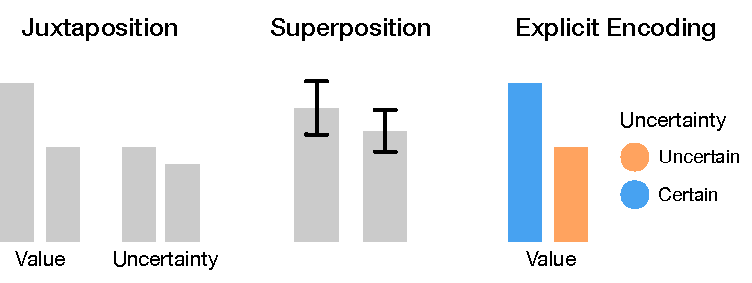
\includegraphics[width=.9\columnwidth]{strategies.pdf}
		\caption{Strategies for encoding uncertainty information along with values. From left to right: encode uncertainty as a separate visualization, overlay uncertainty information with separate glyphs in the same visualization, or encode uncertainty with a separate visual channel on the same glyphs.}
		\label{fig:strategies}
	\end{figure}
}